% !TEX root = ../ds3.tex


%%%%%%%%%%%%%%%%%%%%%%%%%%%%%%%%%%%%%%%%%%%%%%%%%%%%%%%%%%%%%%%%%%%%%%%%%%%%%%%
%%%%%%%%%%%%%%%%%%%%%%%%%%%%%%%%%%%%%%%%%%%%%%%%%%%%%%%%%%%%%%%%%%%%%%%%%%%%%%%
\section{Introduction}
\label{sec:intro}
%%%%%%%%%%%%%%%%%%%%%%%%%%%%%%%%%%%%%%%%%%%%%%%%%%%%%%%%%%%%%%%%%%%%%%%%%%%%%%%
%%%%%%%%%%%%%%%%%%%%%%%%%%%%%%%%%%%%%%%%%%%%%%%%%%%%%%%%%%%%%%%%%%%%%%%%%%%%%%%

%%%%%%%%%%%%%%%%%%%%%%%%%%%%%%%%%%%%%%%%%%%%%%%%%%%%%%%%%%%%%%%%%%%%%%%%%%%%%%%
\begin{frame}{Introduction}
\textcolor{blue}{TODO graphical introduction}
\end{frame}
%%%%%%%%%%%%%%%%%%%%%%%%%%%%%%%%%%%%%%%%%%%%%%%%%%%%%%%%%%%%%%%%%%%%%%%%%%%%%%%

%%%%%%%%%%%%%%%%%%%%%%%%%%%%%%%%%%%%%%%%%%%%%%%%%%%%%%%%%%%%%%%%%%%%%%%%%%%%%%%
\begin{frame}{Empirical Risk Minimization (ERM)}
    \alert{Goal}: from examples $(x_1, y_1), \dots, (x_n, y_n)$ learn a function $h: \bbR^p \rightarrow R$ such that 
    \begin{equation*}
        h(x_{n+1}) \simeq y_{n+1}
    \end{equation*}

\pause

\alert{Ideally}, for a given loss function $L$ :
\begin{equation*}
    h^* \in \argmin_{h \in \cH} \underbrace{\bbE [L(h(x), y)]}_{\text{Risk}}
\end{equation*}

\pause 

\alert{In practice}:
\begin{equation*}
    h^* 
    \in 
    \argmin_{h \in \cH} 
    \underbrace{\sum_i^n L(h(x_i), y_i)}_{\text{Empirical risk}}
\end{equation*}

\end{frame}
%%%%%%%%%%%%%%%%%%%%%%%%%%%%%%%%%%%%%%%%%%%%%%%%%%%%%%%%%%%%%%%%%%%%%%%%%%%%%%%

%%%%%%%%%%%%%%%%%%%%%%%%%%%%%%%%%%%%%%%%%%%%%%%%%%%%%%%%%%%%%%%%%%%%%%%%%%%%%%%
\begin{frame}{Examples of ERM in Practice}
Let $X = [x_1, \dots, x_n]^\top \in \bbR^{n \times p}$ (design matrix)\\
\medskip
%
Linear Regression:
%
\begin{align*}
    w^*
    \in 
    \argmin_{w \in \bbR^p}
    \frac{1}{2} \norm{y - Xw}^2
\end{align*}
%
\pause 

Logistic Regression:
%
\begin{align*}
    w^*
    \in 
    \argmin_{w \in \bbR^p}
    \sum_{i=1}^{n} \log(1 + \exp(- y_i X_{i, :} w))
\end{align*}

\pause 

\begin{itemize}
    \item Boils down to convex optimization problems!
\end{itemize}
\end{frame}
%%%%%%%%%%%%%%%%%%%%%%%%%%%%%%%%%%%%%%%%%%%%%%%%%%%%%%%%%%%%%%%%%%%%%%%%%%%%%%%

%%%%%%%%%%%%%%%%%%%%%%%%%%%%%%%%%%%%%%%%%%%%%%%%%%%%%%%%%%%%%%%%%%%%%%%%%%%%%%%
\begin{frame}{Convex analysis tools I}
    \textcolor{blue}{gradients}
\end{frame}
%%%%%%%%%%%%%%%%%%%%%%%%%%%%%%%%%%%%%%%%%%%%%%%%%%%%%%%%%%%%%%%%%%%%%%%%%%%%%%%


%%%%%%%%%%%%%%%%%%%%%%%%%%%%%%%%%%%%%%%%%%%%%%%%%%%%%%%%%%%%%%%%%%%%%%%%%%%%%%%
\begin{frame}{Convexity I}
    \begin{definition}[Convex function]
    $f: \bbR^p \rightarrow \bbR$ is convex if and only if, $ \forall u, v \in \bbR^p$, $ \forall \lambda \in [0, 1]$:
    \begin{align*}
        f(\lambda u + (1 - \lambda) v)
        \leq 
        \lambda f(u) + (1 - \lambda) f(v)
    \end{align*}
    \end{definition}
    
    \centering
    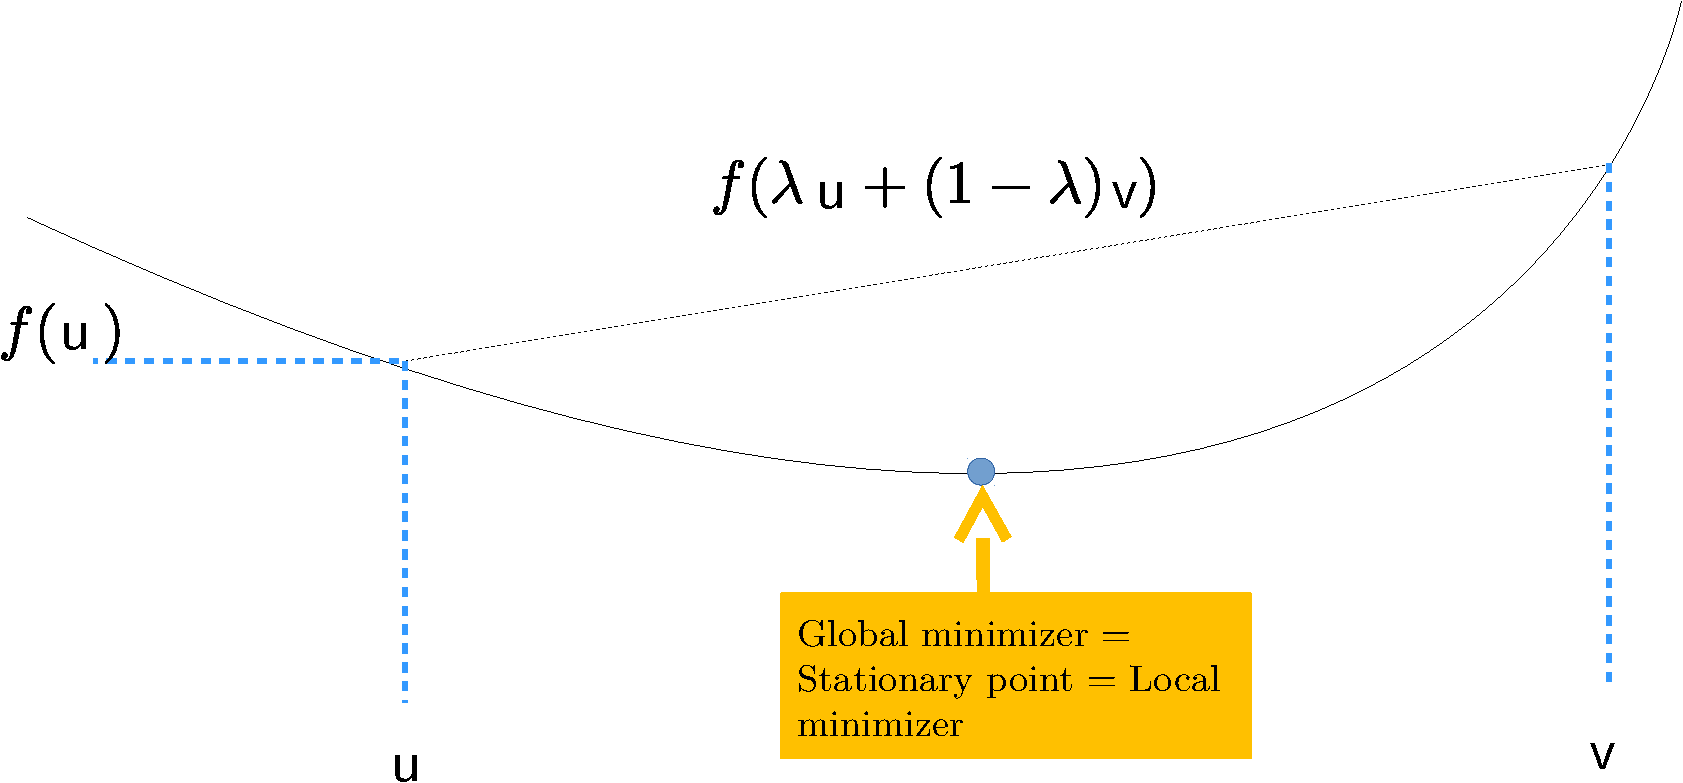
\includegraphics[width=30em]{convexity_1-crop}


\end{frame}
%%%%%%%%%%%%%%%%%%%%%%%%%%%%%%%%%%%%%%%%%%%%%%%%%%%%%%%%%%%%%%%%%%%%%%%%%%%%%%%

%%%%%%%%%%%%%%%%%%%%%%%%%%%%%%%%%%%%%%%%%%%%%%%%%%%%%%%%%%%%%%%%%%%%%%%%%%%%%%%
\begin{frame}{Convexity II}
    \begin{proposition}[Convex differentiable function]
        $f: \bbR^p \rightarrow \bbR$ is convex if and only if, $ \forall u, v \in \bbR^p$:
        \begin{align*}
            f(v)
            \geq 
            f(u) 
            + \langle \nabla f(u), v - u \rangle 
    \end{align*}
    \end{proposition}

    \centering
    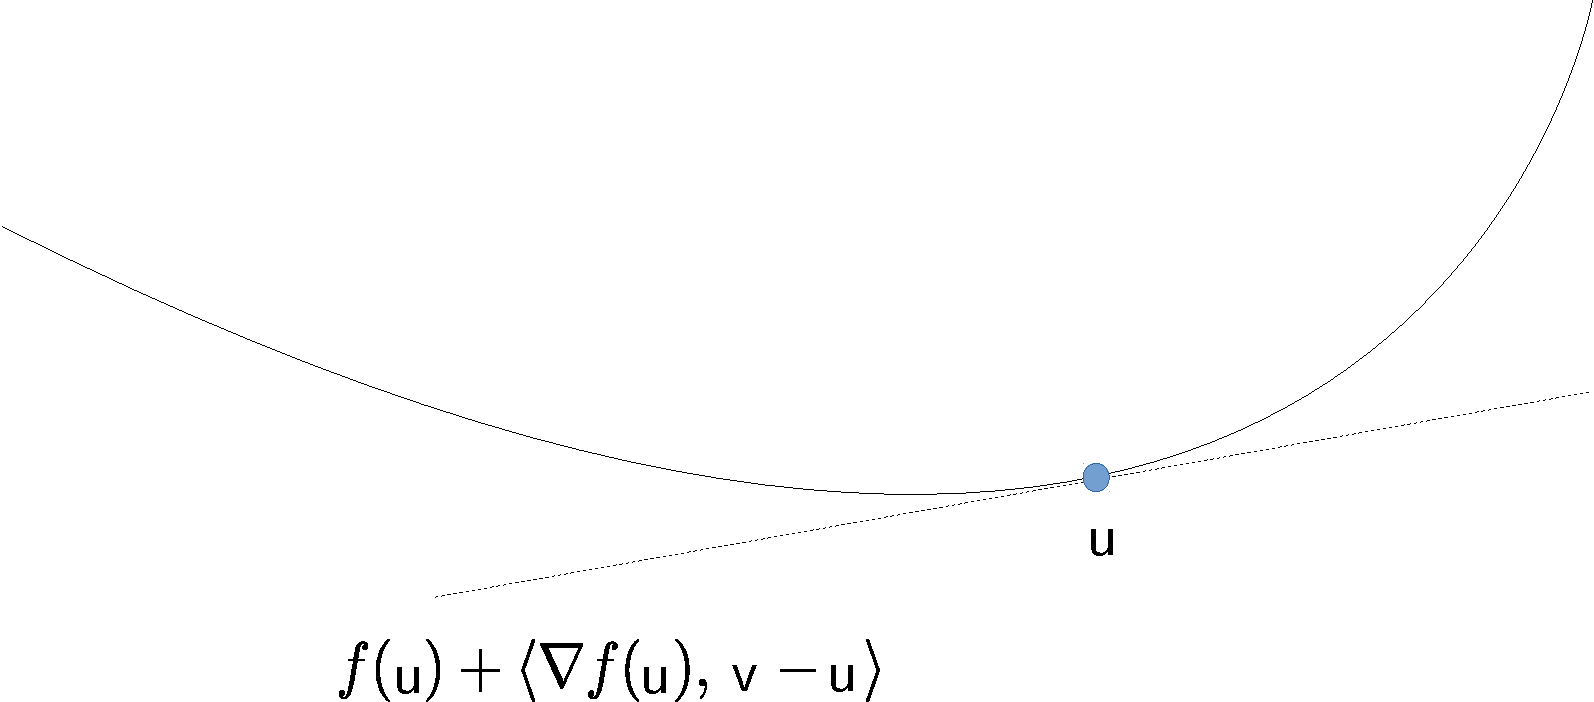
\includegraphics[width=30em]{convexity_2-crop}
    
\end{frame}
%%%%%%%%%%%%%%%%%%%%%%%%%%%%%%%%%%%%%%%%%%%%%%%%%%%%%%%%%%%%%%%%%%%%%%%%%%%%%%%

%%%%%%%%%%%%%%%%%%%%%%%%%%%%%%%%%%%%%%%%%%%%%%%%%%%%%%%%%%%%%%%%%%%%%%%%%%%%%%%
\begin{frame}{Convexity III}
    \begin{proposition}[Convex twice differentiable function]
        $f: \bbR^p \rightarrow \bbR$ is convex if and only if, $ \forall u\in \bbR^p$:
        \begin{align*}
            \nabla^2 f(u) \succeq 0
        \end{align*}
    \end{proposition}
    
    \centering
    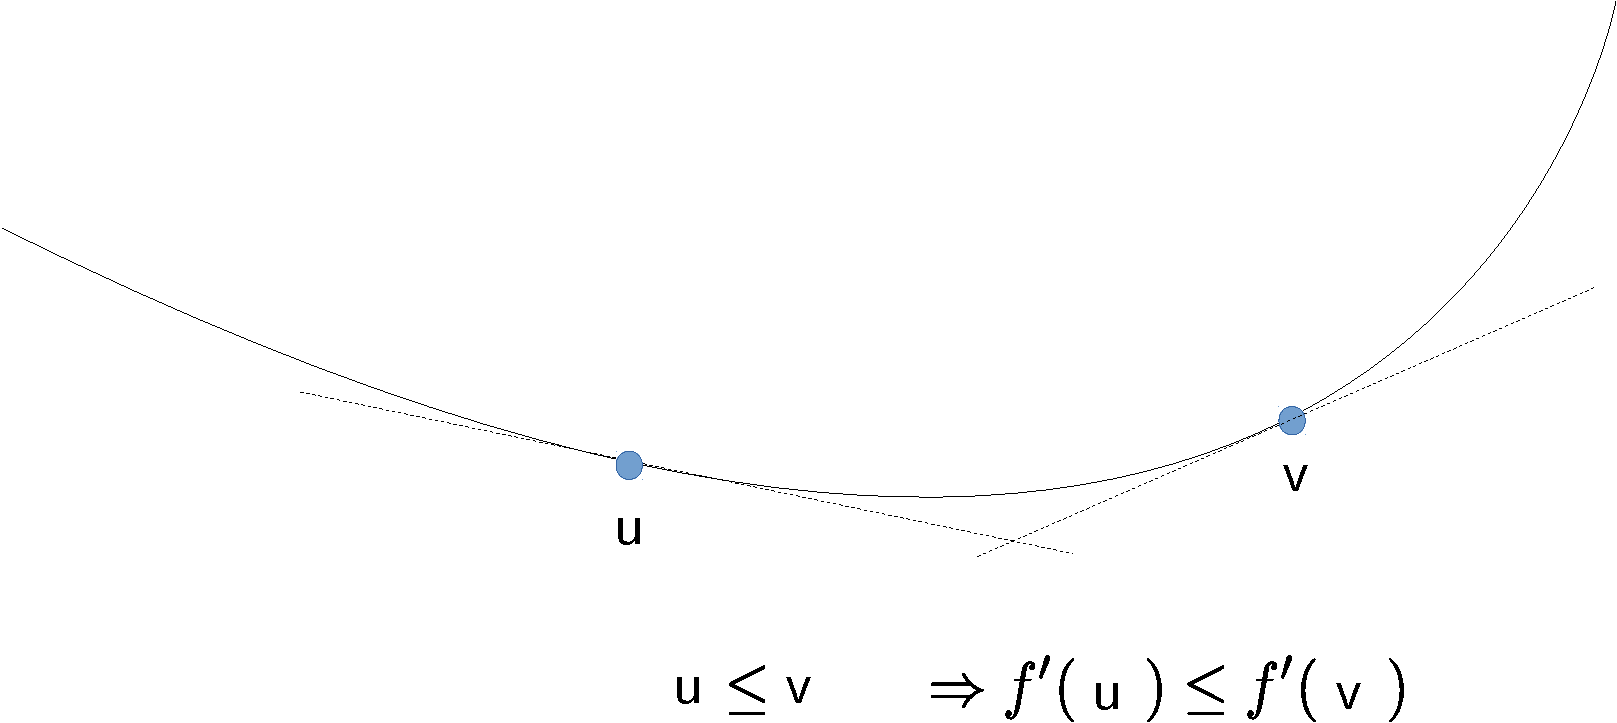
\includegraphics[width=30em]{convexity_3-crop}
\end{frame}
%%%%%%%%%%%%%%%%%%%%%%%%%%%%%%%%%%%%%%%%%%%%%%%%%%%%%%%%%%%%%%%%%%%%%%%%%%%%%%%



%%%%%%%%%%%%%%%%%%%%%%%%%%%%%%%%%%%%%%%%%%%%%%%%%%%%%%%%%%%%%%%%%%%%%%%%%%%%%%%
\begin{frame}{Strong Convexity I}
    \begin{definition}[Strongly convex function]
    $f: \bbR^p \rightarrow \bbR$ is $\mu$-strongly convex if and only if, $ \forall u, v \in \bbR^p$:
        \begin{align*}
            f(v)
            \geq 
            f(u) 
            + \langle \nabla f(u), v - u \rangle 
            + \frac{\mu}{2} \normin{v - u}^2
    \end{align*}
    \end{definition}
\end{frame}
%%%%%%%%%%%%%%%%%%%%%%%%%%%%%%%%%%%%%%%%%%%%%%%%%%%%%%%%%%%%%%%%%%%%%%%%%%%%%%%

%%%%%%%%%%%%%%%%%%%%%%%%%%%%%%%%%%%%%%%%%%%%%%%%%%%%%%%%%%%%%%%%%%%%%%%%%%%%%%%
\begin{frame}{Strong Convexity II}
    \begin{proposition}[Strongly convex twice differentiable function]
        $f: \bbR^p \rightarrow \bbR$ is $\mu$-strongly convex if and only if, $ \forall u \in \bbR^p$:
        \begin{align*}
            \nabla^2 f(u) \succeq \mu \Id_p
        \end{align*}
    \end{proposition}

\end{frame}
%%%%%%%%%%%%%%%%%%%%%%%%%%%%%%%%%%%%%%%%%%%%%%%%%%%%%%%%%%%%%%%%%%%%%%%%%%%%%%%

%%%%%%%%%%%%%%%%%%%%%%%%%%%%%%%%%%%%%%%%%%%%%%%%%%%%%%%%%%%%%%%%%%%%%%%%%%%%%%%
\begin{frame}{Smoothness}
    \begin{definition}[Smoothness]
        $f: \bbR^p \rightarrow \bbR$ is $L$-smooth if and only if, $\nabla f$ is $L$-Lipschitz
        $ \forall u, v \in \bbR^p$
        \begin{align*}
            \norm{\nabla f (u) - \nabla f (v)}
            \leq 
            L \norm{u - v}
        \end{align*}
        in particular this implies
        \begin{align*}
            f(v)
            \leq 
            f(u)
            + \langle \nabla f (u) , v - u \rangle
            + \frac{L}{2} \normin{v - u}^2
        \end{align*}
    \end{definition}
    \centering
    
\includegraphics[width=30em]{smoothness-crop}
\end{frame}
%%%%%%%%%%%%%%%%%%%%%%%%%%%%%%%%%%%%%%%%%%%%%%%%%%%%%%%%%%%%%%%%%%%%%%%%%%%%%%%
